\section{Convolutional neural network}

Many of the approaches, described in the Section \ref{sec:spacerecognition}, that uses NN for the classification of objects use already extracted features from the image. These features are obtained from the database but the process of the extraction is not explicitly defined in the articles. Another common approach was to use a predefined set of features, which are then measured using traditional methods. For this reason, the majority of approaches choose to use MLP when designing the architecture of their network.

In \cite{Burke2019}, authors used one region-based network, which performed the task of object localization and classification. The convolutional subnetwork extracted the features from the image that it considered important, therefore no predefined features were needed. In our work we are following the same concept. We propose a convolutional neural network that classifies images based on features extracted from them using convolutional layers.

%However as explained in \cite{Burke2019}, it proved to be beneficial to use only one network for classification, and object localization and let the network extract features it needs as well. In our work, we decided to follow the same concept. We are using a convolutional neural network to extract the features from images and classify them into various classes. 

%In this section, we will describe the architecture of the network, we designed specifically for this task. To compare the performance of our network to state-of-the-art networks, we will also deploy the ResNet network. 

In this section, we will describe two CNN architectures: LeNet and ResNet. The former network was an inspiration for the architecture we designed specifically for this thesis, which will be explained in greater detail in the next chapter. The latter is used to compare the performance of our network to state-of-the-art networks. 


\subsection{LeNet}

LeNet \cite{lenet5} is one of the first successful applications of CNN in computer vision. The model was designed to recognize handwritten digits. The model achieved impressive results, matching the performance of SVM.

The structure of the network (Figure \ref{img:lenet}) could be grouped into two parts: convolutional and dense block. 

The convolutional block is made up of two convolutional layers, each followed by a subsampling layer. Both convolutional layers use 5x5 kernel and sigmoid activation. As for the subsampling layer, it operates with a 2x2 kernel with a stride of 2 and performs an average pooling operation. Before passing the output volume to the dense block, it must be flattened to a 1D vector, which is the aim of the third convolutional layer. As this last layer performs convolution with a 5x5 kernel on the input volume with a spatial size of 5x5, the output is a one-dimensional vector.  

The dense block consists of two fully-connected layers. The first layer contains 84 neurons that are connected to each node in the flattened vector from the previous layer. The last layer has 10 neurons, which represent the number of classes (digits from 0 to 9). After the last fully-connected layer, softmax activation is used to produce class scores. 

\begin{figure}[h]
    \centering
    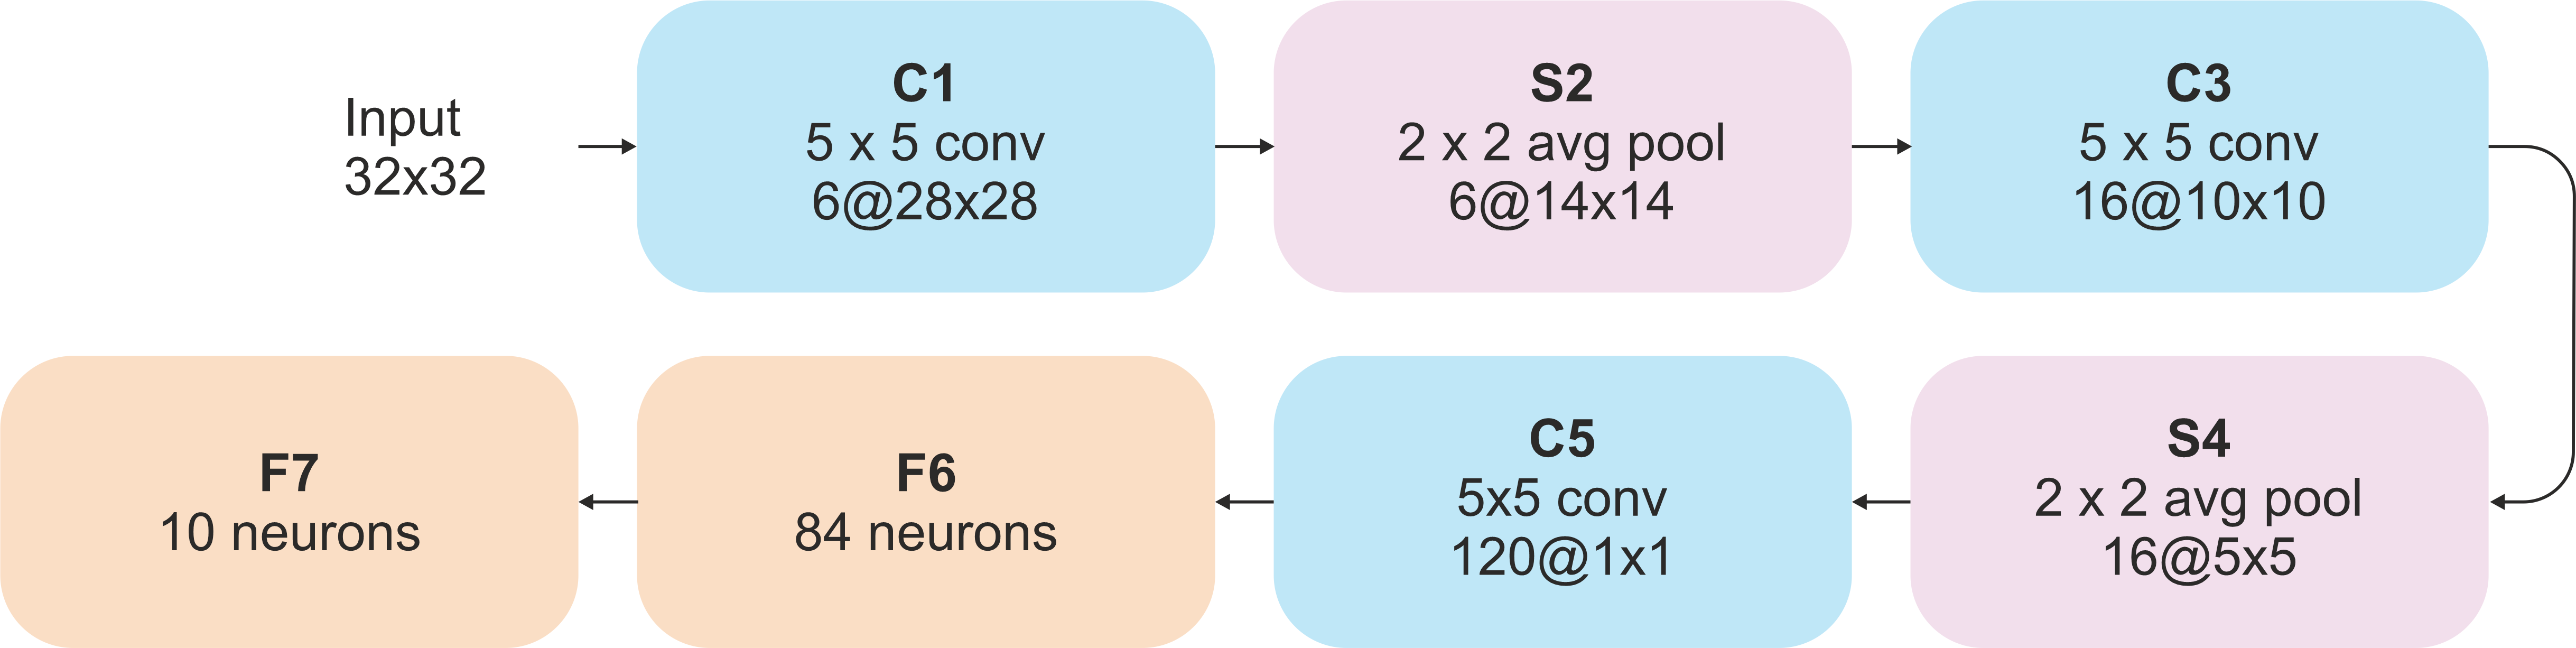
\includegraphics[width=.8\textwidth]{images/lenet.png}
    \caption{The LeNet architecture.}
    \label{img:lenet}
\end{figure}

\subsection{ResNet}

Residual neural network \cite{resnet2015} is a specific type of neural network that is constructed using residual blocks, which contain special residual connections. These blocks allow the network to be significantly deeper while also reducing the problem of vanishing gradient. Even with the increased depth, the residual network proved to be easier to optimize. After winning first place in ILSVRC \cite{ILSVRC} in 2015, the ResNet has become the default choice for using CNNs in practice. This is one of the reasons why we have decided to use it, to compare our network to state-of-the-art models.  

The topology of the residual block (Figure \ref{img:resblock0}) consists of two 3x3 convolutions, each followed by batch normalization and RELU activation. The main feature of the residual block is the residual connection, which adds the block input with the output directly before the last RELU activation. To be able to do the addition, the spatial size of the two convolutional layers needs to match the size of the input. The number of feature maps also needs to be the same, but this issue can be easily solved with a 1x1 convolution performed on the input. 

The concept of residual connections is based on the idea that stacking the layers to make the network deeper shouldn't reduce the performance, since we could just stack layers that don't change the value of the input data and we would get the same result. 
We will explain this using the Figure \ref{img:resblock0}. Let's assume that the mapping we want the network to learn is $f(x)$ with the input to the block denoted as $x$. With the residual block, the network only needs to learn the residual mapping $f(x) - x$, since the input $x$ will be added to the output. If the block needs to learn the identity mapping $f(x) = x$, it could simply just output zeros. This way, the block outputs the same data it received and therefore doesn't degrade the performance of the network with a deeper topology. 

\begin{figure}[h]
    \centering
    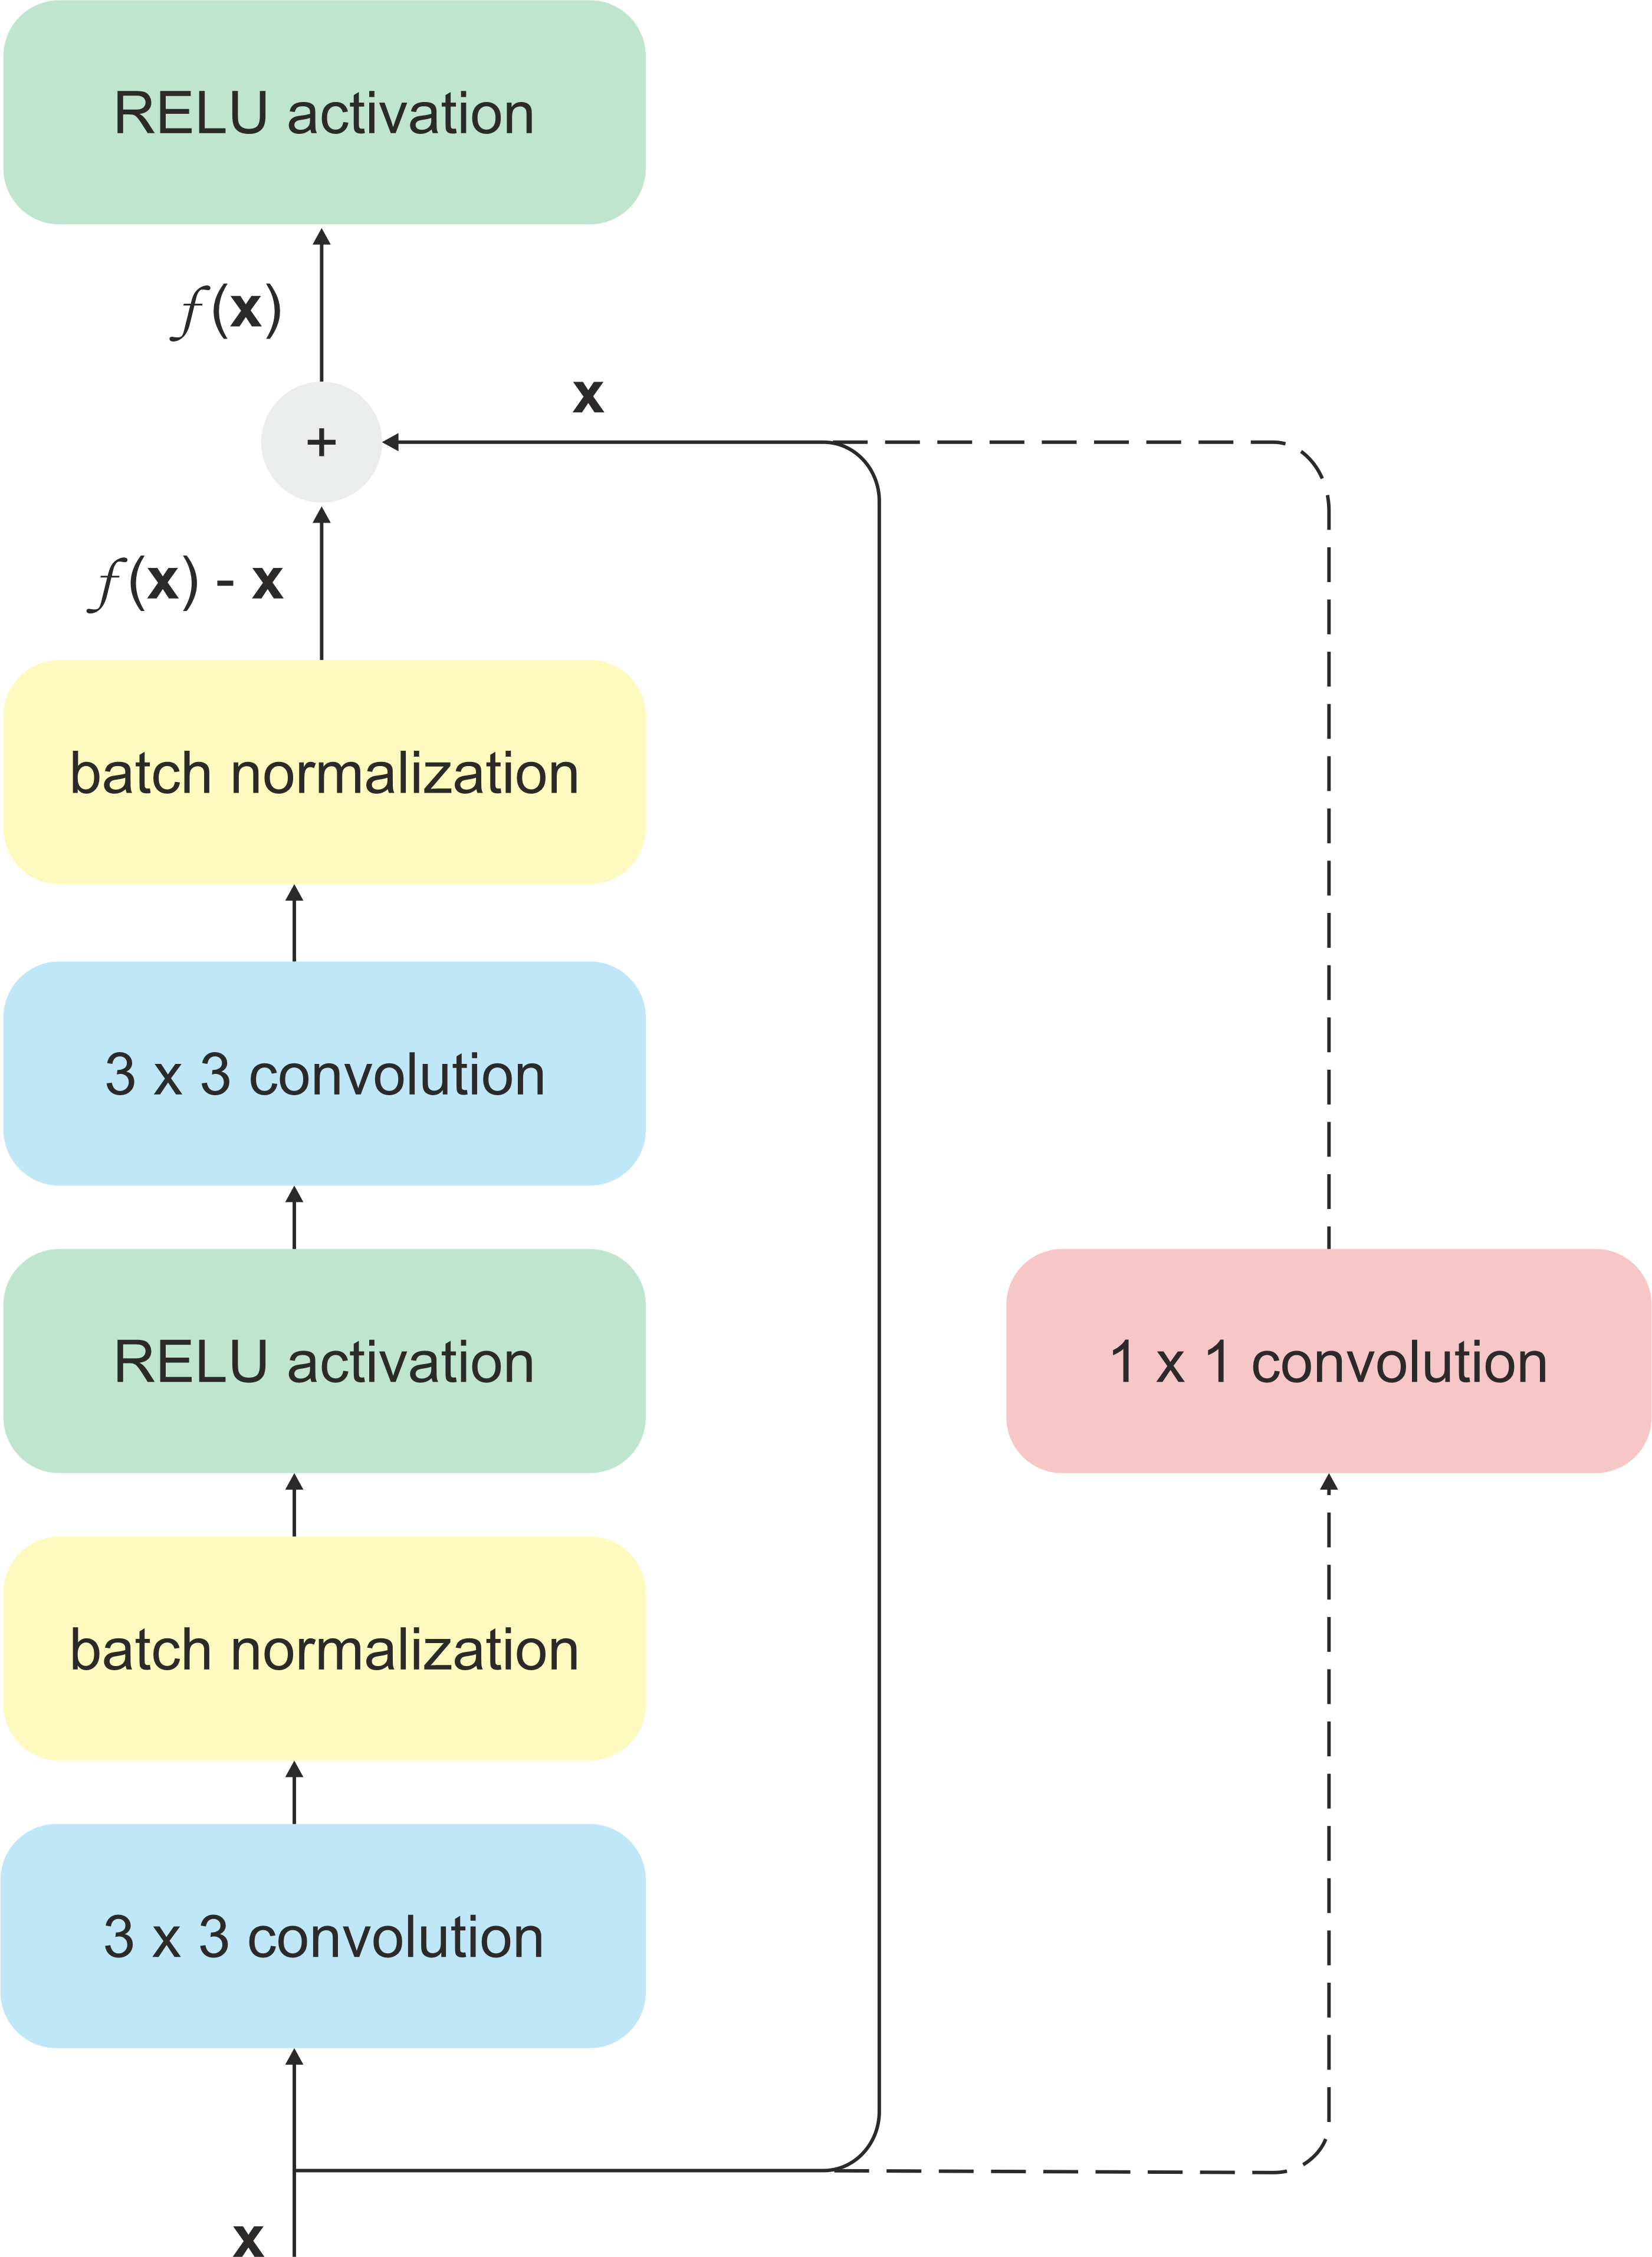
\includegraphics[width=0.4\textwidth]{images/residualblock.png}
    \caption{The structure of Resnet residual block.}
    \label{img:resblock0}
\end{figure}

By changing the number of filters and residual blocks, we can create different versions of ResNet models (ResNet-18, ResNet-152). In our work we are using ResNet-18 (Figure \ref{img:resnet18}) which consists of 18 layers. 


\begin{figure}[h]
    \centering
    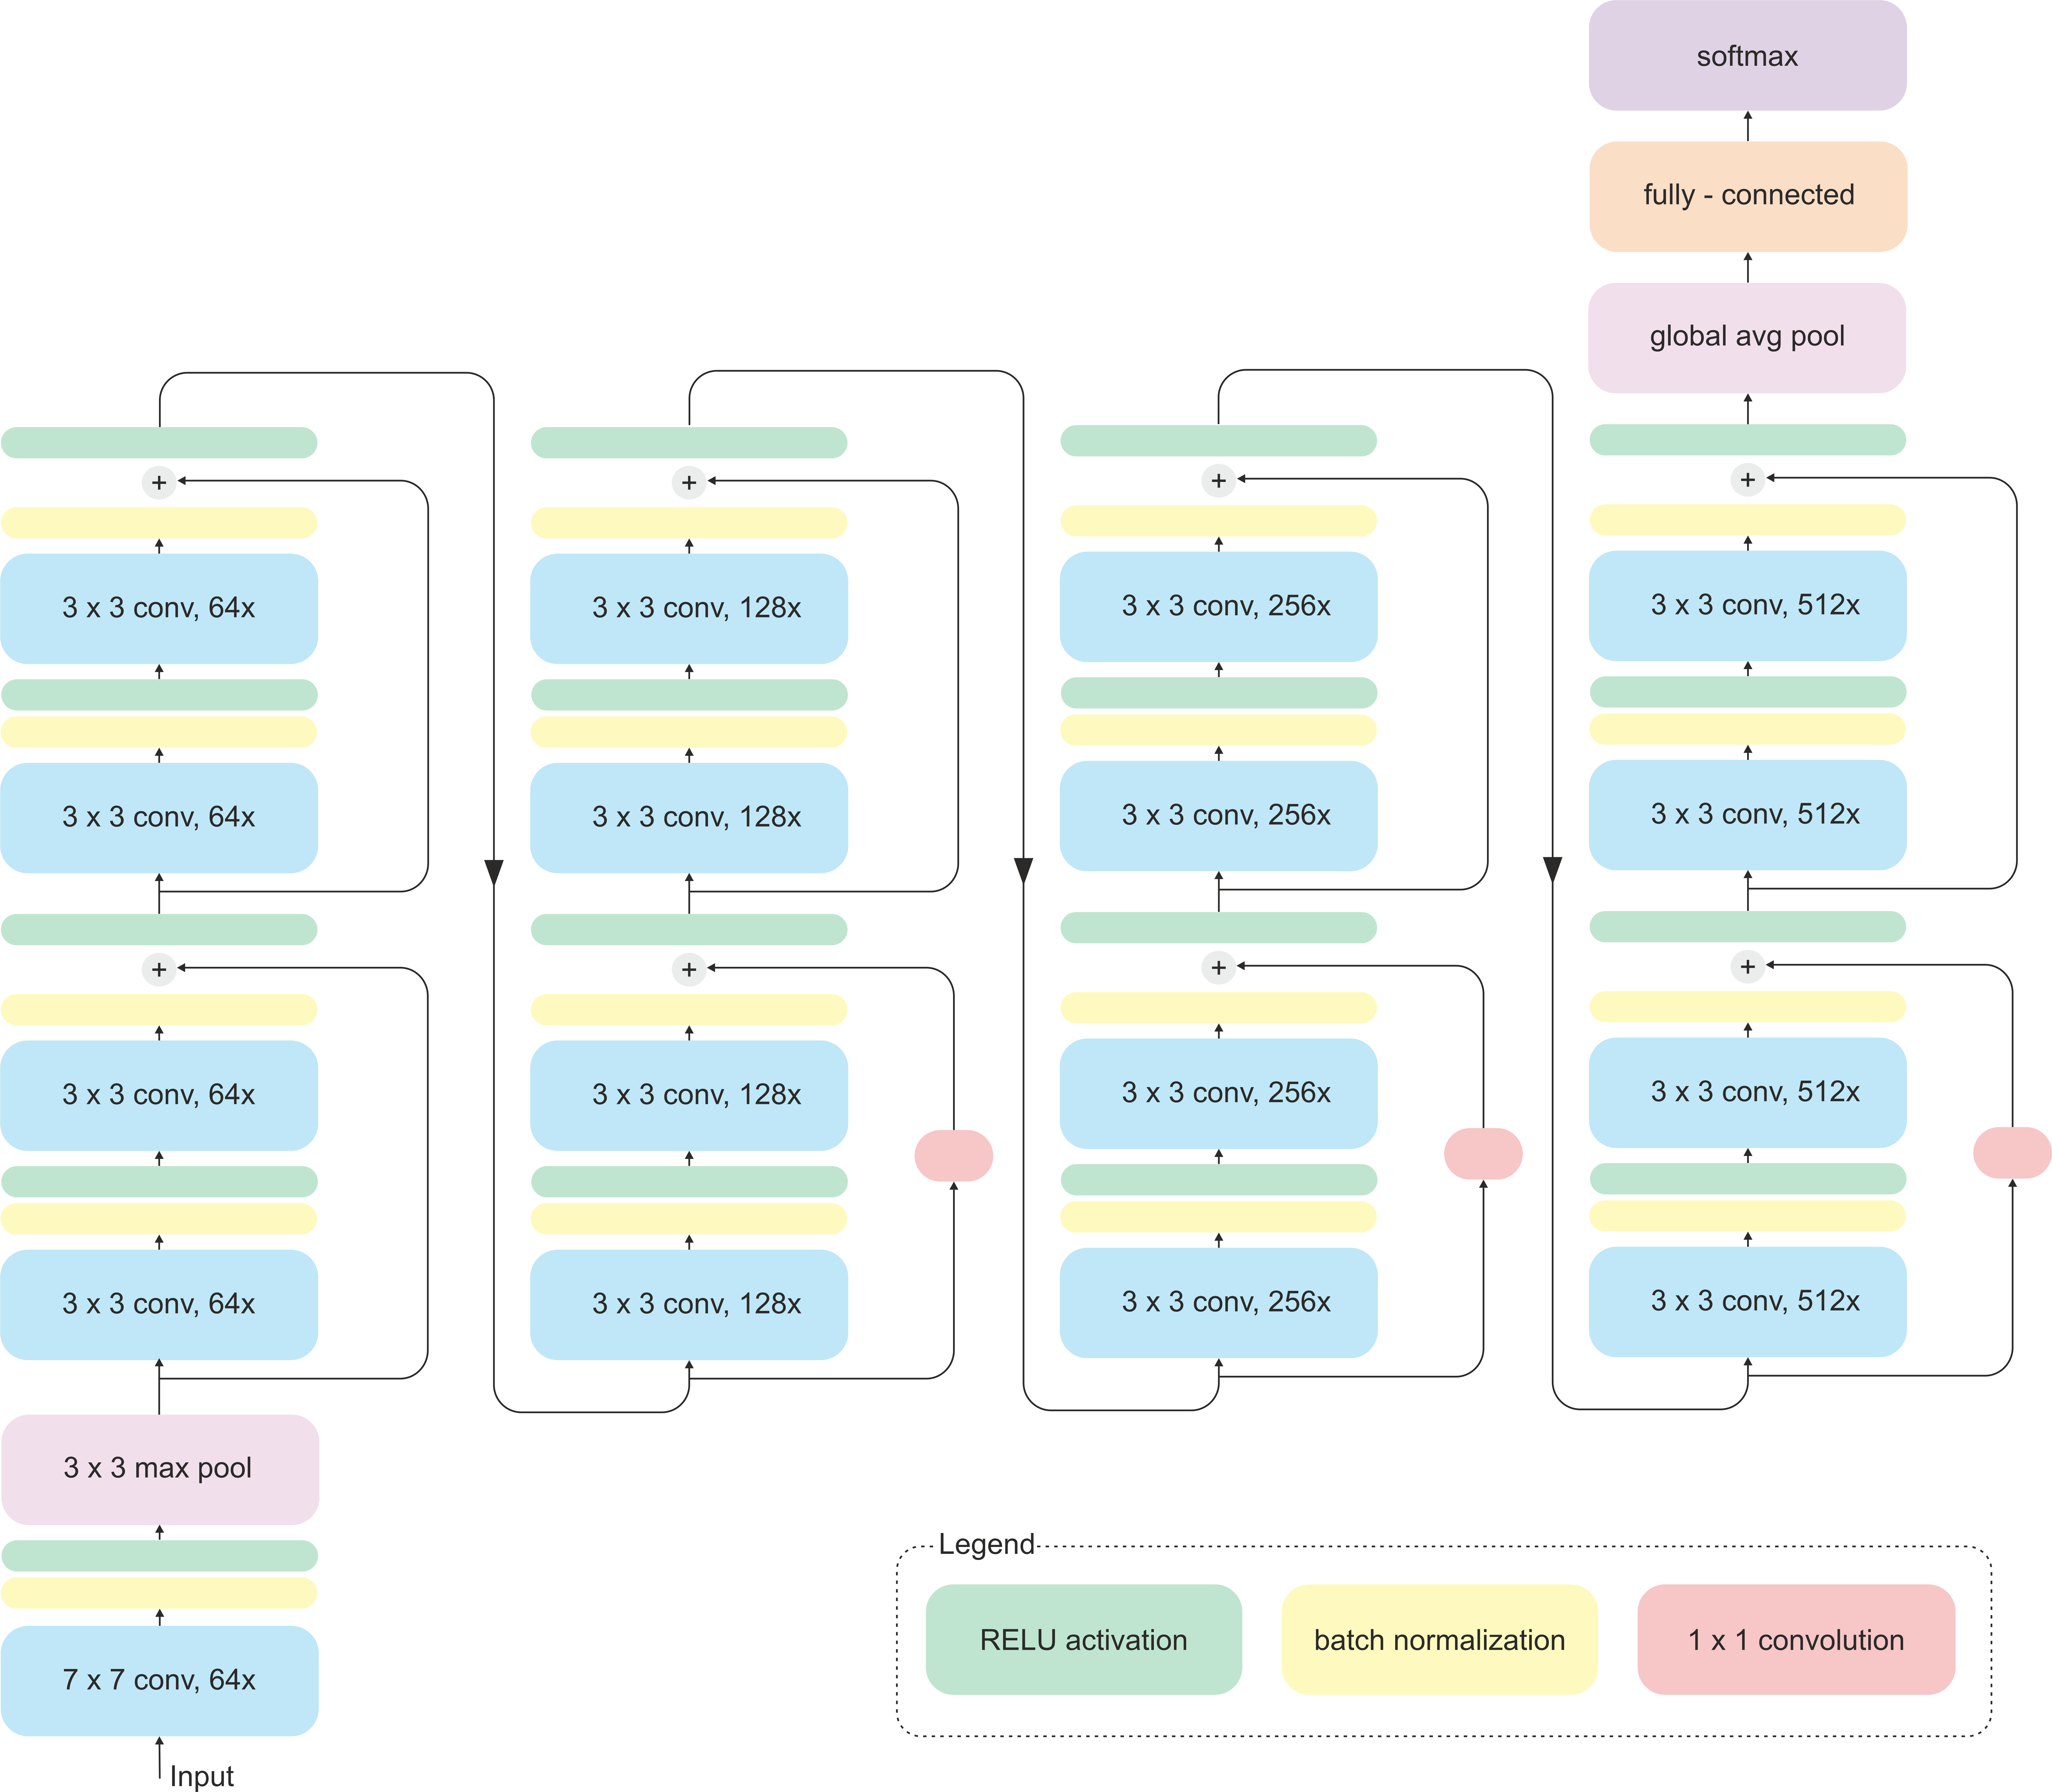
\includegraphics[width=0.8\textwidth]{images/resnet18.png}
    \caption{The ResNet-18 architecture.}
    \label{img:resnet18}
\end{figure}
